\chapter{Evaluierung}\label{evaluierung}

\section{Implementierung} \label{Tests}
Die Implementierung des Min-Conflicts-Embedders und der Automatismus zum Lösen von Bindungs- und Routinganforderungen wurden in X10 \cite{x10} geschrieben. Desweiteren wurde das vom Lehrstuhl \grqq Hardware-Software-Co-Design\grqq (Universität Erlangen-Nürnberg) entwickelte CoNoC-Framework in die parallele, objektorientierte Programmiersprache transformiert. Es wurden zwei Arten von Taskgraphen erstellt und diese mithilfe des Simulators \textit{invadeSIM} \cite{invadeSIM}  ausgewertet.

%Die Implementierung des CSP-Solver (Backtracking-Algorithmus [\ref{Backtracking}] und Min-Conflicts-Algorithmus [\ref{minConflicts}]) und der Variablenheuristiken (MWO [\ref{MWO}], MBO [\ref{MBO}], MaxHops [\ref{MaxHops}]) erfolgte in der Programmiersprache Java. Für die Simulation eines Network-On-Chips (NoC) wurde das vom Lehrstuhl \grqq Hardware-Software-Co-Design\grqq (Universität Erlangen-Nürnberg) entwickelte CoNoC-Framework verwendet. Die Taskgraphen wurden mit Hilfe des Programms \textit{Task Graphs for Free} \cite{tgff} erstellt.  \\
%\\




\section{Testumgebung} \label{Testumgebung1} 
Die Testumgebung besteht aus einem NoC, der  eine Breite und eine Länge von 10 Kacheln hat. Die Unit- bzw LinkAttribute sind folgendermaßen:
\\
\begin{itemize}
\item UnitAttribute
\begin{itemize}
\item TypeAttribute\\
Die Hälfte aller Kacheln sind vom Ressourcentyp 0. Der Rest ist Ressourcentyp 1.
\item UnitWorkloadAttribute\\
Die Workload einer jeden Kachel beträgt 100.

\end{itemize}
\item LinkAttribute
\begin{itemize}
\item LinkBandwithAttribute\\
Die Bandbreite eines jeden Links beträgt 10.
\end{itemize}
\end{itemize}

Für die Randbedingungen wurden folgende Vereinfachungen getroffen:
\begin{itemize}
\item TaskConstraint
\begin{itemize}
\item TypeConstraint\\
Die Hälfte aller Tasks sind vom Ressourcentyp 0. Der Rest ist Ressourcentyp 1.
\item TaskWorkloadConstraint \\
Jeder Task benötigt eine Nutzlast von 100.
\end{itemize}
\item CommunicationConstraint
\begin{itemize}
\item BandwidthConstraint\\
Jede Communication benötigt eine Bandbreite von 5.
\item MaxHopConstraint\\
Die maximale Distanz zwischen zwei miteinander kommunizierenden Tasks beträgt immer 3.
\end{itemize}
\end{itemize}

Es werden zwei Arten von Taskgraphen näher untersucht. Zum einen ein sequentieller Taskgraph (Abbildung \ref{fig:seq}) bei dem jeder Task die gleiche Anzahl an Kommunikationen besitzt und zum anderen ein parallelisierter Taskgraph (Abbildung \ref{fig:par}) bei dem mehrere Kommunikationen von einem Task ausgehen. Die Tasks, die die Kommunikation empfangen, arbeiten hierbei zeitgleich weiter. Für beide Taskgrapharten werden jeweils 5, 7 und 10 Tasks erstellt.
\begin{figure}[H]\centering
  \includegraphics[width = 120mm]{bilder/sequentiell.jpg}
  \caption{Sequentieller Taskgraph: Ein Kreis repräsentiert einen Task. Ein Rechteck stellt eine Kommunikation dar.
  }\label{fig:seq}
\end{figure}

\begin{figure}[H]\centering
  \includegraphics[width = 70mm]{bilder/parallel.jpg}
  \caption{Parallelisierter Taskgraph: Ein Kreis repräsentiert einen Task. Ein Rechteck stellt eine Kommunikation dar.}\label{fig:par}
\end{figure}

\section{Auswertung} \label{Auswertung} 




\begin{figure}
\centering
        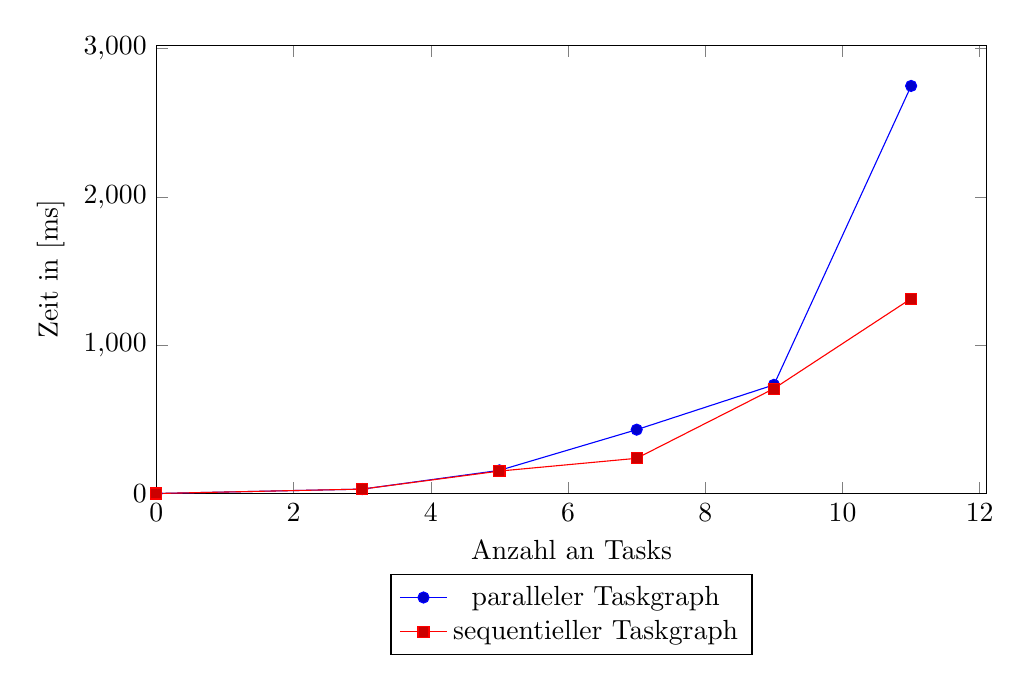
\begin{tikzpicture}
         \pgfplotsset{every axis legend/.append style={at={(0.5,-0.18)}, anchor=north}}
                \begin{axis}[xmin=0,ymin=0,
                xlabel={Anzahl an Tasks},
                ylabel={Zeit in [ms]},
                width=1.0\textwidth,
      height=0.6\textwidth]
%                \addplot [domain=0:80, samples=60]{1750.763223011357};
                        \addplot coordinates {
                        (0, 0)
                        (3, 29.628)
                        (5, 155.8845)
                        (7, 430.3)
                        (9, 732.4)
                       (11, 2747.662)
};

                        \addplot coordinates {
                        (0, 0)
                         (3, 29.628)
                        (5, 151.2)
                        (7, 237.3)
                        (9, 707.2)
                       (11, 1313.9)
};

         \legend{paralleler Taskgraph, sequentieller Taskgraph}
                \end{axis}
        \end{tikzpicture}
\caption{Vergleich der unterschiedlichen Terminierungsverfahren an einem Beispiel
geringerer Komplexität als in Beispiel \ref{Terminierungsverfahren2}}
\label{Terminierungsverfahren1}
\end{figure}  





\begin{figure}
\centering
        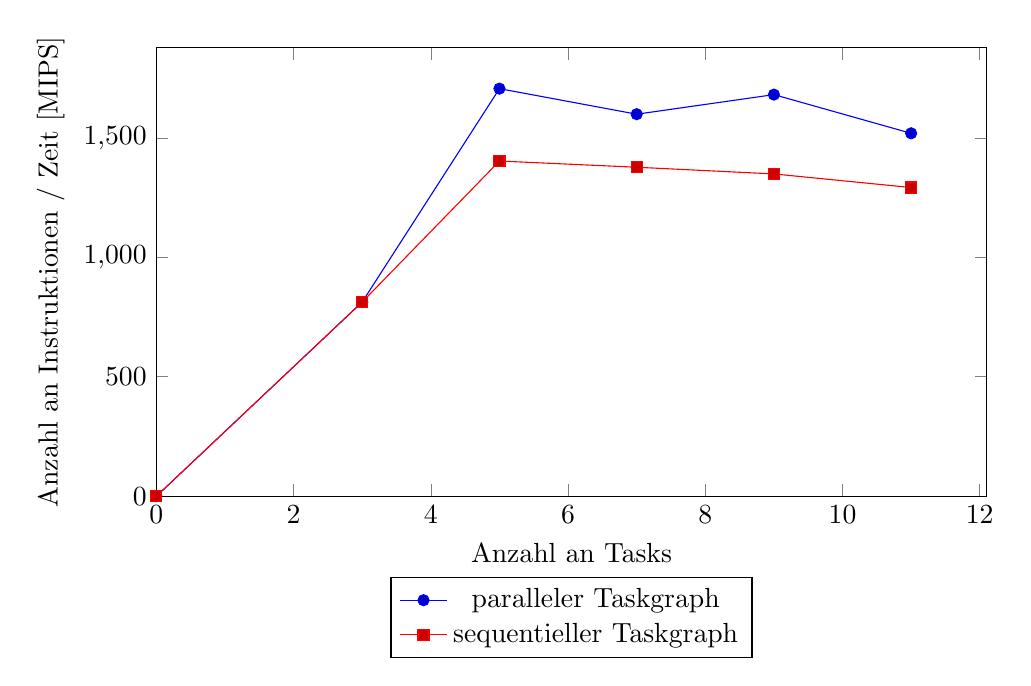
\begin{tikzpicture}
         \pgfplotsset{every axis legend/.append style={at={(0.5,-0.18)}, anchor=north}}
                \begin{axis}[xmin=0,ymin=0,
                xlabel={Anzahl an Tasks},
                ylabel={Anzahl an Instruktionen / Zeit [MIPS]},
                width=1.0\textwidth,
      height=0.6\textwidth]
%                \addplot [domain=0:80, samples=60]{1750.763223011357};
                        \addplot coordinates {
                        (0, 0)
                        (3, 813)
                        (5, 1706)
                        (7, 1599)
                        (9, 1681)
                       (11, 1519)
};

                        \addplot coordinates {
                        (0, 0)
                         (3, 813)
                        (5, 1403)
                        (7, 1377)
                        (9, 1349)
                       (11, 1292)
};

        \legend{paralleler Taskgraph, sequentieller Taskgraph}
                \end{axis}
        \end{tikzpicture}
\caption{Vergleich der unterschiedlichen Terminierungsverfahren an einem Beispiel
geringerer Komplexität als in Beispiel \ref{Terminierungsverfahren2}}
\label{Terminierungsverfahren1}
\end{figure}  



%\begin{itemize}
%%\begin{tabular}{ll}
%
%\item $b_{ressource}$: \qquad $\forall t_i \in T:$ $t_i.$ressourceType $\in$ \{0,1\} \\
% 50 \% der Tasks benötigen Ressourcentyp 0  und 50 \% der Tasks Ressourcentyp 1.
%
%\item $b_{isOK}$: \qquad  $\forall k_i \in K:$ $k_i.$fehlerfrei = $True$ \\
%Alle Kacheln sind funktionsfähig.
%%\end{itemize}
%
%
%\item $b_{capacity}$: \qquad  $\forall$ $t_i \in T$: $t_i.$ressourceRequirements = 100\\
%Jeder Task benötigt die Kachel zu 100 \%. Das heißt, das auf einer Kachel nur ein Task laufen kann.
%
%
%
%\item $b_{distance}$: \qquad  $\forall t_i \in T$: $t_i$.HopLimit $\in \{1,2,3\}$\\
%Das HopLimit ist gleichverteilt zwischen 1 und 3.
%
%
%
%\item $b_{routing}$: \qquad   $\forall c_i \in C$: $c_i$.bandwidth $\cdot$ 2   =  $\forall l_j \in L$: $l_j.capacity$. \\
%Die Bandbreite jedes Kommunikationsknoten ist die Hälfte der Kapazität eines jeden Links.
%
%%\end{tabular}
%\end{itemize}
%\ \\
%Tasks können mit bis zu vier eingehenden und bis zu fünf ausgehenden Kommunikationsknoten verbunden sein.
%\ \\
%\subsection{Testumgebung 2} \label{Testumgebung2}
%Die Testumgebung 2 unterscheidet sich von Testumgebung 1 einzig bei der Rahmenbedingung $b_{routing}$.
%
%\begin{itemize}
%\item  $b_{routing}$: \qquad   $\forall c_i \in C$: $c_i$.bandwidth $\cdot$ 10   =  $\forall l_j \in L$: $l_j.capacity$. \\
%Die Bandbreite jedes Kommunikationsknoten ist ein Zehntel der Kapazität eines jeden Links.
%\end{itemize}




%Die zum Evaluieren der Algorithmen verwendeten Taskgraphen wurden mit dem Programm
%Task Graphs for Free [DRW98] generiert. Die Tasks k¨onnen mit bis zu drei
%eingehenden und zwei ausgehenden Kommunikationsknoten verbunden sein und werden
%zuf¨allig einem von drei Ressourcentypen zugeteilt. Der maximale Abstand der zugeh
%¨origen Tasks kann dabei zuf¨allig zwischen eins und neun gew¨ahlt werden.



%In diesem Kapitel soll dargelegt werden, ob Forward-Checking (Kapitel \todo{kapitel}) seine Daseinsberechtigung hat. Um dies festzustellen, wurde eine Testumgebung erstellt. Die Testumgebung besteht aus 50 verschiedenen NoCs, die jeweils eine Breite von 10 und Länge von 10 Kacheln haben. Eine Kachel ist entweder vom Ressourcentyp 0 oder den Ressourcentyp 1. Der Ressourcentyp der Kacheln wurde zufällig und gleichverteilt bestimmt. Auf den NoCs laufen zu Beginn der Einplanung keine Anwendungen. 50 \% der Tasks benötigen Ressourcentyp 0 ($t_i$.ressourceType = 0) und 50 \% der Tasks Ressourcentyp 1 ($t_i$.ressourceType = 1). Alle Kacheln sind funktionsfähig, d.h. die Nebenbedingung $b_{isOK}$ ist für jede vollständige Zuweisung erfüllt. Für die Nebenbedingung $b_{capacity}$ ist zu beachten, dass jeder Task $t_i \in T$ die Kachel zu 100 \% ($t_i.$ressourceRequirements = 100) benötigt. D.h. das auf einer Kachel nur ein Task laufen kann. Die Nebenbedingung $b_{routing}$ wurde folgendermaßen vereinfacht: $\forall c_i \in C$: $c_i$.bandwidth $\cdot$ 2   =  $\forall l_j \in L$: $l_j.capacity$. Die Bandbreite jedes Kommunikationsknoten ist die Hälfte der Kapazität eines jeden Links. Um die beiden Varianten vergleichen zu können, wurden jeweils die gleichen Taskgraphen verwendet. Jeder Taskgraph wurde auf die 50 NoCs eingeplant. Der Durchschnittswert von der Anzahl der Einplanungen für jeden Taskgraphen wurden gebildet, wobei die jeweils 15, die am meisten Einplanungsversuche, und die 15, die am wenigsten Einplanungsversuche pro Runde benötigten, verworfen wurden. Mit einer Runde ist hierbei gemeint, dass der Taskgraph auf die 50 NoCs  \\

%\section{Vergleich zwischen Backtracking mit und ohne Forward-Checking} \label{BTFC}
%
%%In diesem Kapitel soll dargelegt werden, ob Forward-Checking (Kapitel \todo{kapitel}) seine Daseinsberechtigung hat. Um dies festzustellen, wurde eine Testumgebung erstellt. Die Testumgebung besteht aus 50 verschiedenen NoCs, die jeweils eine Breite von 10 und Länge von 10 Kacheln haben. Eine Kachel ist entweder vom Ressourcentyp 0 oder den Ressourcentyp 1. Der Ressourcentyp der Kacheln wurde zufällig und gleichverteilt bestimmt. Auf den NoCs laufen zu Beginn der Einplanung keine Anwendungen. 50 \% der Tasks benötigen Ressourcentyp 0 ($t_i$.ressourceType = 0) und 50 \% der Tasks Ressourcentyp 1 ($t_i$.ressourceType = 1). Alle Kacheln sind funktionsfähig, d.h. die Nebenbedingung $b_{isOK}$ ist für jede vollständige Zuweisung erfüllt. Für die Nebenbedingung $b_{capacity}$ ist zu beachten, dass jeder Task $t_i \in T$ die Kachel zu 100 \% ($t_i.$ressourceRequirements = 100) benötigt. D.h. das auf einer Kachel nur ein Task laufen kann. Die Nebenbedingung $b_{routing}$ wurde folgendermaßen vereinfacht: $\forall c_i \in C$: $c_i$.bandwidth $\cdot$ 2   =  $\forall l_j \in L$: $l_j.capacity$. Die Bandbreite jedes Kommunikationsknoten ist die Hälfte der Kapazität eines jeden Links. Um die beiden Varianten vergleichen zu können, wurden jeweils die gleichen Taskgraphen verwendet. Jeder Taskgraph wurde auf die 50 NoCs eingeplant. Der Durchschnittswert von der Anzahl der Einplanungen für jeden Taskgraphen wurden gebildet, wobei die jeweils 15, die am meisten Einplanungsversuche, und die 15, die am wenigsten Einplanungsversuche pro Runde benötigten, verworfen wurden. Mit einer Runde ist hierbei gemeint, dass der Taskgraph auf die 50 NoCs  \\
%%\\
%
%Wie man in Abbildung \ref{fig:forwardChecking} sehen kann, benötigt man sehr viel weniger Einplanungsversuche, falls Forward-Checking (FC) zur Anwendung kommt. Wenn Forward-Checking benutzt wird, wird nur auf Kacheln einplant, die keine Randbedingung $b_i \in B$ verletzen. Vor allem die Randbedingung $b_{distance}$ verringert hierbei den Suchraum enorm. Ohne FC ist der Suchraum so groß wie  das komplette NoC. Die Maximalzahl an Einplanungen (bei 15 Tasks) betrug ohne FC 1.183.082, mit FC hingegen nur 56.385. So gab es beim Verfahren ohne FC bis zu 20 mal mehr Einplanungsversuche als mit der Verwendung von FC. Dies spiegelt in etwa das Verhältnis der Größe der Domänen in beiden Varianten wieder. %Bei der Verwendung von Backtracking ohne FC (BoFC) sind alle Kacheln in der Domäne $D_{BoFC}$ und bei der Verwendung von Backtracking mit FC (BmFC) sind nur die Kacheln  in der Domäne $D_{BmFC}$, die alle Nebenbedingungen $b_i \in B$ erfüllen, erlaubt.
%
%
%%\begin{figure}[H]\centering
%%  \includegraphics[width = 150mm]{bilder/forwardChecking.jpg}
%%  \caption{Vergleich zwischen Backtracking mit Forward--Checking und ohne Forward--Checking }\label{fig:forwardChecking}
%%\end{figure}
%
%\section{Vergleich der Variablenordnungsverfahren}
%
%In diesem Abschnitt werden die Variablenordnungsverfahren aus Kapitel \ref{variableOrdering} verglichen. Hierbei wurden die drei vorgestellten Variablenordnungsverfahren (Minimal-Bandwidth-Ordering, Minimal-Width-Ordering, MaxHops) auf die Testfälle aus Abschnitt \ref{Tests} angewandt und ausgewertet. \\
%\\
%Der Testfall 1 (Abschnitt \ref{Testumgebung1}) wurde in Abbildung \ref{fig:ordering2Links} und der Testfall 2 (Abschnitt \ref{Testumgebung2}) in Abbildung \ref{fig:ordering10Links} ausgewertet. Wie zu erwarten war, steigt der Lösungsaufwand mit der Anzahl an Tasks. Zum einen zeigt es sich, dass die schwer zu erfüllende $b_{routing}$-Bedingung aus Testfall 1 einen maßgeblichen Anteil an der Anzahl der Einplanungen auf die Kacheln besitzt. Es werden bis zu 67 mal mehr Einplanungen beim Testfall 1  als beim Testfall 2 getätigt. Zum anderen erkennt man, dass die verschiedenen Testumgebungen keinen Einfluss auf die Rangfolge der Ordnungsverfahren hat. In beiden Testumgebungen benötigt Minimal-Bandwidth-Ordering (MBO) die wenigsten Einbettungen. Mit einem eher kleinen Abstand folgt Minimal-Width-Ordering (MWO) auf Rang zwei. Sehr viel mehr Einbettungen benötigt MaxHops im Vergleich zu MBO und MWO. Deshalb ist MaxHops besonders für große Taskgraphen nicht empfehlenswert.
%
%%\begin{figure}[H]\centering
%%  \includegraphics[width = 150mm]{bilder/ordering3.jpg}
%%  \caption{Vergleich zwischen den drei vorgestellten Variablenordnungsverfahren. Testumgebung 1 stammt aus Abschnitt \ref{Testumgebung1}.}\label{fig:ordering2Links}
%%\end{figure}
%
%%\begin{figure}[H]\centering
%%  \includegraphics[width = 150mm]{bilder/variablenordnung10nachrichtenProLink.jpg}
%%  \caption{Vergleich zwischen den drei vorgestellten Variablenordnungsverfahren. Testumgebung 2 stammt aus Abschnitt \ref{Testumgebung2}.}% Die Variablenordnungen wurden in Testumgebung 2 (Abschnitt \ref{Testumgebung2}) ausgewertet. 
%%  \label{fig:ordering10Links}
%%\end{figure}
%
%%Wie man in Abbildung \ref{fig:ordering} erkennt, benötigen MWO und MBO annähernd die gleiche Anzahl an Einbettungen. Das MaxHops Verfahren fällt gegenüber den anderen zwei vorgestellten Verfahren ab. Dies liegt daran, dass MaxHops nicht nach Anzahl der Abhängigkeiten (MWO und MBO) sortiert, sondern nach der Größe der maximalen HopLimits. So ist es bei MaxHops möglich, dass ein Task der zu Beginn eingeplant werden soll, auch mit Tasks am Ende der Einplanungsordnung in Verbindung steht. \\
%%\\
%\ \\
%Obwohl MBO die wenigsten Einbettungen benötigt, ist er nicht empfehlenswert. MBO benötigt für die Berechnung der Taskreihenfolge eine Zeitkomplexität von $\mathcal O(n^k)$ ($n$ Anzahl der Tasks und $k$ minimale Bandbreite). MWO und MaxHops haben lediglich eine Zeitkomplexität  von $\mathcal O(n^2)$ ($n$ Anzahl der Tasks). Tabelle \ref{table:Zeit} und die dazugehörige Abbildung \ref{fig:Zeit} zeigen die Berechnungsdauer für die Ordnungsverfahren. Es zeigt sich, dass die Berechnungszeit für MBO zu lange dauert, um es in der Praxis anzuwenden. Deshalb ist MWO als guter Kompromiss zwischen wenigen Einplanungen und kurze Berechnungsdauer empfehlenswert.
%%Als schnellstes Ordnungsverfahren stellte sich MBO bei den Tests heraus. Der Abstand zu MWO ist nicht besonders groß. Gegen MBO spricht, dass es eine sehr hohe Zeitkomplexität von $\mathcal O(n^k)$ ($n$ Tasks und $k$ maximale Bandbreite) im Gegensatz zu MWO $\mathcal O(n^2)$ hat. Aus diesem Grund ist MWO dem MBO vorzuziehen.\\
%\\
%\begin{table}[H]\centering
%\begin{tabular} {c | c | c | c}
%\ & MWO & MBO & MaxHops \\
%\hline
%5 Tasks & 6 ms & 6 ms & 6 ms \\
%7 Tasks & 6 ms & 12 ms & 6 ms \\
%10 Tasks & 7 ms & 18 ms & 7 ms \\
%12 Tasks & 8 ms & 199 ms & 7 ms \\
%15 Tasks & 8 ms & 13.250 ms & 9 ms
%\end{tabular}
%\caption{Zeitdauer (in Millisekunden) für die Berechnung der Variablenreihenfolge.} 
%\label{table:Zeit}
%\end{table}
%
%%die Tasks im Gegensatz zu MWO und MBO nicht zwangsläufig durch Kommunikationsknoten verbunden sind. So ist es möglich, dass mehrere Tasks den 
%%\begin{figure}[H]\centering
%%  \includegraphics[width = 150mm]{bilder/ZeitmessungVariablenordnung.jpg}
%%  \caption{Zeitdauer für die Variablenordnungsverfahren}\label{fig:Zeit}
%%\end{figure}
%
%
%
%
%\section{Vergleich zwischen Min-Conflicts und Backtracking}
%
%In diesem Abschnitt wird Min-Conflicts (Abschnitt \ref{minConflicts}) mit dem Backtracking-Verfahren (Abschnitt \ref{Backtracking}) verglichen. Backtracking verwendet hierbei Forward-Checking (Abschnitt \ref{ForwardChecking}) und das Variablenordnungsverfahren Minimal-Width-Ordering (MWO, Abschnitt \ref{MWO}). Die Ergebnisse aus Testumgebung 1 (Abschnitt \ref{Testumgebung1}) werden in Abbildung \ref{fig:MinConflictTest1} und die Ergebnisse aus Testumgebung 2 (Abschnitt \ref{Testumgebung2}) werden in Abbildung \ref{fig:MinConflictsTest2} dargestellt.  \\
%\\
%Der Min-Conflicts-Algorithmus darf pro Testfall 100 Durchgänge durchlaufen. Das heißt, es können alle Tasks 100 mal neu und zufällig gesetzt werden. Pro Durchgang ist es 500 mal möglich, einen konflikterzeugenden Task auszuwählen und die Konflikte zu lösen bzw. zu minimieren. Falls es dennoch zu keiner gültigen Belegung der Tasks kommt, wird der Testfall als \textit{nicht gelöst} bewertet.\\
%\\
%Die gestrichelte Linie in beiden Abbildungen zeigt auf, mit welcher Wahrscheinlichkeit der Min-Conflicts-Embedder eine Lösung für das gegebene Problem findet. Die Wahrscheinlichkeit sinkt mit der Anzahl an Tasks. Besonders in Abbildung \ref{fig:MinConflictsTest2} sieht man deutlich, wie die Wahrscheinlichkeit, dass der Min-Conflicts-Embedder eine Lösung findet, schwindet. Die Erfolgswahrscheinlichkeit beim Backtracking-Verfahren ist jedoch immer bei 100 \%. \\
%\\
%Die durchgezogenen Linien stellen den Mittelwert der Einbettungen auf den Kacheln graphisch dar. Es werden hierbei nur erfolgreiche Einbettungsversuche gewertet.\\
%\\
%In Abbildung \ref{fig:MinConflictTest1} erkennt man, dass die Erfolgswahrscheinlichkeit für das Min-Conflicts-Verfahren deutlich sinkt. So findet der Min-Conflicts-Embedder bei der Anzahl von 15 Tasks nur in 18 \% der Fälle eine Lösung. Der Grund liegt in den schwer erfüllbaren Bedingungen der Testumgebung 1, insbesondere Bedingung $b_{routing}$. \\
%\\
%Der Verlauf der Einbettungsfunktion zeigt Folgendes: Bei einer geringen Anzahl an Tasks ist das Backtracking- und das Min-Conflicts-Verfahren annähernd gleich. Steigt die Anzahl der Tasks\footnote{das zu lösende Problem wird schwieriger}, so benötigt der Min-Conflcits-Embedder erheblich mehr Einbettungen. Der Knick an der Stelle zwischen zehn und zwölf Tasks lässt sich damit erklären, dass die Erfolgsquote von Min-Conflicts in dieser Auswertungsspanne erheblich gesunken ist. %Die NoC Noc-Architekturen ausgewertet die viele Lösungen befinden
%
%% Die wenigen erfolgreichen Einplanungsversuche verfälschen das Ergebnis, da nur die lassen keinen statistischen zu \todo{Formulierung wenige erfolgreiche Einplanungsversuche. Bei den wenigen . }
%
%%Zuerst wird die Erfolgsquote der Min-Conflicts-Heuristik (Kapitel \refminConflicts) untersucht. Hierbei werden die Testfälle aus Abschnitt \ref{Tests} wieder verwendet. Der Algorithmus darf pro Testfall 40 Durchgänge durchlaufen, das heißt es können alle Tasks 40 mal neu und zufällig gesetzt werden. Pro Durchgang ist es 200 mal möglich einen konflikterzeugenden Task auszuwählen und die Konflikte zu lösen bzw. zu minimieren. Falls es dennoch zu keiner Lösung kommt, wird der Testfall als \textit{nicht gelöst} bewertet. In Abbildung \ref{fig:MinConflictErfolgsquote} ist zu erkennen, dass es mit der ansteigender Zahl an Tasks die Min-Conflicts-Heuristik seltener eine Lösung findet, obwohl eine Lösung vorhanden ist. Das Backtracking-Verfahren findet jedoch immer eine Lösung, falls eine vorhanden ist.
%
%%\begin{figure}[H]\centering
%%  \includegraphics[width = 150mm]{bilder/MinConflicts2Links.jpg}
%%  \caption{Vergleich zwischen Backtracking mit Minimal-Width-Ordering (MWO) und Min-Conflicts. Testumgebung 1 stammt aus Abschnitt \ref{Testumgebung1}. \\
%%  Die durchgezogenen Linien geben die Einbettungen auf den Kacheln an. \\
%%  Die gestrichelte Linie gibt die Erfolgswahrscheinlichkeit der Einbettung an.}\label{fig:MinConflictTest1}
%%\end{figure}
%\ \\
%Abbildung \ref{fig:MinConflictsTest2} stellt die Auswertung der Testumgebung 2 (Abschnitt \ref{Testumgebung2}) dar. Die Erfolgsquote ist hierbei höher als bei Abbildung \ref{fig:MinConflictsTest2}. Das liegt daran, dass es mehr Lösungen auf den Network-on-Chip (NoC) gibt. Der Min-Conflicts-Embedder schneidet aber wiederum viel schlechter als der Backtracking-Embedder ab. 
%%In Abbildung \ref{fig:VergleichMinConflictBacktracking} wird das Backtracking- mit dem Min-Conflicts-Verfahren verglichen. Hierbei werden nur erfolgreiche Einbettungsversuche gewertet. Im Backtracking-Verfahren wurde Forward-Checking verwendet. Zuvor wurden die Tasks mit Hilfe dem Variablenordnungsverfahern MWO geordnet. Wie auf der Abbildung zu erkennen ist, steigt die Anzahl der Einbettungsversuche bei Backtracking stärker als bei Min-Conflicts an. Dies sieht auf den ersten Blick positiv aus. Jedoch muss die viel geringere Erfolgsquote von Min-Conflicts berücksichtigt werden. So sollte bei der gewählten Testumgebung (Abschnitt \ref{Tests}) ab einer Anzahl von 10 Tasks der Min-Conflicts als CSP-Solver nicht mehr ausgewählt werden. Min-Conflicts eignet sich vor allem als Reparaturverfahren. Wenn schon eine Lösung gefunden wurde, aber eine von einem Task benutzte Kachel defekt wird. Hier kann Min-Conflicts eine Lösung mit wenigen Einbettungsversuchen finden.
%
%%\begin{figure}[H]\centering
%%  \includegraphics[width = 150mm]{bilder/MinConflicts10Links.jpg}
%%  \caption{Vergleich zwischen Backtracking mit Minimal-Width-Ordering (MWO) und Min-Conflicts. Testumgebung 2 stammt aus Abschnitt \ref{Testumgebung2}. Die durchgezogenen Linien geben die Einbettungen auf den Kacheln an. Die gestrichelte Linie gibt die Erfolgswahrscheinlichkeit der Einbettung an.}\label{fig:MinConflictsTest2}
%%\end{figure}
%\ \\
%Die Evaluierung hat ergeben, dass das Min-Conflicts-Verfahren insbesondere für schwer zu lösende Probleme ungeeignet ist. Die Verwendung des Min-Conflicts-Verfahren für die Einbettungen einer Anwendung in einem Network-on-Chip (NoC) ist nicht zu empfehlen, falls es sich um ein schwer zu erfüllendes Problem handelt. Min-Conflicts eignet sich jedoch als Reparaturverfahren \cite{cspsolvingRepairMethod}, wenn bereits eine Lösung gefunden wurde, aber eine von einem Task benutzte Kachel defekt wird. In diesem Fall kann Min-Conflicts eine Lösung mit wenigen Einbettungsversuchen finden.
